\switchcolumn[1]*
\begin{figure}[!h]
  \centering
  \begin{minipage}[t]{0.495\linewidth}
    \centering
    $\cvec$\vspace{1ex}
    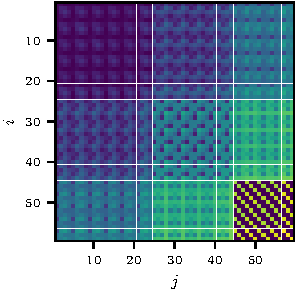
\includegraphics[width=\linewidth]{../kfs/plots/synthetic_cvec_ggn.pdf}
  \end{minipage}
  \hfill
  \begin{minipage}[t]{0.495\linewidth}
    \centering
    $\rvec$\vspace{1ex}
    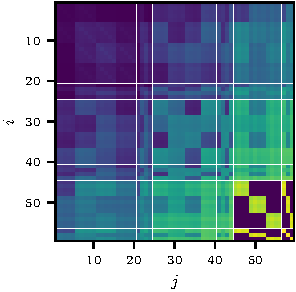
\includegraphics[width=\linewidth]{../kfs/plots/synthetic_rvec_ggn.pdf}
  \end{minipage}
  \\
  \begin{minipage}[t]{0.495\linewidth}
    \centering
    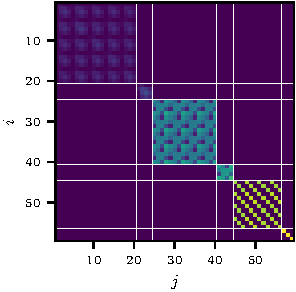
\includegraphics[width=\linewidth]{../kfs/plots/synthetic_cvec_ggn_bda.pdf}
  \end{minipage}
  \hfill
  \begin{minipage}[t]{0.495\linewidth}
    \centering
    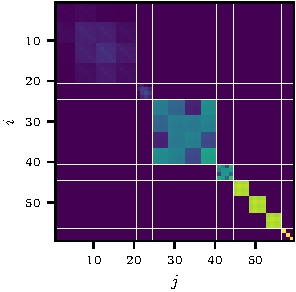
\includegraphics[width=\linewidth]{../kfs/plots/synthetic_rvec_ggn_bda.pdf}
  \end{minipage}
  \caption{\textbf{The GGN of a neural net exhibits block structure.}
    We visualize the GGN and its block-diagonal approximation using different flattening schemes.
    We use synthetic data ($N=100$) on an MLP with three fully-connected layers (5-4-4-3) and ReLU activations and square loss.
    The GGN blocks are visually highlighted with white lines.
    The left column uses $\cvec$-flattening, the right column $\rvec$-flattening.
    Plots produced with \repofile{plots/synthetic_fisher}
    (this is not a typo; the Fisher and GGN are closely related as we will see in \Cref{subsec:connection-ggn-fisher}).
  }\label{fig:ggn-block-structure}
\end{figure}

\switchcolumn[0]
Consider the empirical risk from above.
The Hessian matrix under a flattening scheme $\vec$ is
\begin{align*}
  \hess_{\vtheta}^{\vec} \gL_{\sD}(\vtheta)
  =
  R
  \sum_{n=1}^N
  \hess_{\vtheta}^{\vec} \ell_n(\vtheta) \in \sR^{D \times D}\,.
\end{align*}
It contains the second-order partial derivatives of $\gL_{\sD}(\vtheta)$ (\Cref{def:vector_hessian}), \ie
\begin{align*}
  [\hess_{\vtheta}^{\vec} \gL_{\sD}(\vtheta)]_{\colored{i},\colored[VectorPink]{j}}
  =
  \frac{\partial^2 \gL_{\sD}(\vtheta)}{\colored{\partial [\vec(\vtheta)]_i} \colored[VectorPink]{\partial [\vec(\vtheta)]_j}}\,.
\end{align*}

\paragraph{Block structure.} Due to the tuple/list structure of $\vtheta$, the Hessian has a block structure (\Cref{fig:hessian-block-structure}).
A block corresponding to parameters $\vtheta^{(k)}, \vtheta^{(l)}$ is
\begin{align*}
  [\hess_{\colored{\vtheta^{(k)}}, \colored[VectorPink]{\vtheta^{(l)}}}^{\vec} \gL_{\sD}]_{i,j}
  =
  \frac{\partial^2 \gL_{\sD}}{\partial [\colored{\vec\left(\vtheta^{(k)}\right)}]_i \partial [\colored[VectorPink]{\vec\left(\vtheta^{(l)}\right)}]_j}\,
\end{align*}
and we usually suppress repeated differentiation arguments, $\hess_{\vtheta^{(k)}}^{\vec} \coloneqq \hess_{\vtheta^{(k)}, \vtheta^{(k)}}^{\vec}$.
With the shorthand $\hess_{k,l}^{\vec} \coloneq \hess_{\vtheta^{(k)}, \vtheta^{(l)}}^{\vec}$,
the Hessian can be written in block form as
\begin{align*}
  \hess_{\vtheta}^{\vec} \gL
  =
  \begin{pmatrix}
    \hess_1^{\vec} \gL
    &
      \hess_{1, 2}^{\vec} \gL
    &
      \cdots
    &
      \hess_{1, L}^{\vec} \gL
    \\
    \hess_{2, 1}^{\vec} \gL
    &
      \hess_2^{\vec} \gL
    &
      \cdots
    &
      \hess_{2, L}^{\vec} \gL
    \\
    \vdots & \cdots & \ddots & \vdots
    \\
    \hess_{L, 1}^{\vec} \gL
    &
      \hess_{L, 2}^{\vec} \gL
    &
      \cdots
    &
      \hess_L^{\vec} \gL
  \end{pmatrix}\,.
\end{align*}
For KFAC, we will only need the block diagonal approximation of this matrix,
\begin{align*}
  \tilde{\hess}_{\vtheta}^{\vec} \gL
  =
  \begin{pmatrix}
    \hess_1^{\vec} \gL & \vzero & \cdots & \vzero
    \\
    \vzero & \hess_2^{\vec} \gL & \ddots & \vdots
    \\
    \vdots & \ddots & \ddots & \vzero
    \\
    \vzero & \cdots & \vzero & \hess_L^{\vec} \gL
  \end{pmatrix}\,.
\end{align*}
\ie, individual blocks $\{ \hess_{\vtheta^{(k)}}^{\vec} \gL_{\sD}(\vtheta)\}_{k=1}^L$.
%%% Local Variables:
%%% mode: latex
%%% TeX-master: "../main"
%%% End:
